\subsubsection{Analysis of a Simple Periodic Structure}
AFM resolution is commonly indicated by reference to structures that are at least locally periodic, for example, in atomic resolution mapping at a solid-liquid interface\cite{fukuma2018atomic}, in identification of recurrent features in a two-dimensional lattice of membrane proteins\cite{bippes2011high, li2006probing}, or the distinction of the two strands of the double helix along a DNA molecule\cite{pyne2014single}. Therefore, we next considered AFM measurements on a periodic soft material. As shown in  Figure~\ref{fig: Wave Compression Plot}, the structure has a wavelength $\lambda = 10nm$ and amplitude, $A_{Sample} = 10nm $. Except when indenting the peak, the AFM tip will contact the structure laterally. This broadens the wave crest similar to the hemisphere, alongside the simultaneous reduction in trough depth, visible when comparing the sharp and blunt tip heat maps shown in Figure \ref{fig: Wave Compression Plot}B, C, respectively. 

%Moreover, increasing indenter-to-surface ratios produces lower indentation forces due to the large contact radius and force distribution. 

Unlike for the hemisphere, the contact produces an inverse relationship in perceived Young's modulus across the scan positions, shown in Figure \ref{fig: Wave Compression Plot}D. At the surface trough, $x/\lambda = 0.5$, the indenter experiences lateral contact from the surface on both sides producing maximum surface interaction and a larger effective stiffness/ Young's modulus. However, the contact radius decreases for scans away from wave trough and forces are distributed laterally. Therefore, Young's modulus decreases proportionally up to the crest at $x/\lambda \approx 0$. As shown in Figure \ref{fig: Hemisphere Compression Plot}E, Young's moduli generally converge true surface at the wave crest. Conversely, at the trough across most of the range, increasing force produces a more significant deviation in perceived Young's modulus.

As shown in Figure\ref{fig: Wave Compression Plot}F, as before, the tip convolution leads to overestimating the FWHM. At sufficiently high forces, the measured FWHM approaches the sample FWHM. However, the much softer gradient compared to the hemisphere indicate lower compression around the wave's midpoint and large force required to indent the slope region. Moreover, Figure \ref{fig: Wave Compression Plot}G shows much less prominent volume variation than the hemisphere. For each indenter, there is only a slight reduction in volume as the indentation force increases, and, unlike the hemisphere, apparent volume is not directly proportional to indenter radius. As volume is measured from the peak to the trough, the composite reduction in trough depth results in a smaller volume as the indenter radius increases from $R/\lambda =0.15$. 

These results, especially  FWHM and volume, indicate that the apparent sharpness of features may increase at higher forces. However, an increase in resolution could be artifactual\cite{morigaki1998analysis}. Spatial resolution in wave-based microscopy is often quantified by considering the spatial frequencies\cite{novotny1998implications,tolan1998evidence,slough1990atomic, morigaki1998analysis}, wave numbers $k$, here expressed in units of $2\pi/\lambda$. We fit data to a Fourier series to quantify the spatial resolution of the contours and show that the same phenomenon occurs for the indented surface. As the surface and contours are symmetric functions, Fourier analysis only requires the cosine terms, modulated by individual amplitude, $A_k$, and frequency, $2\pi k$, given by, 

\begin{equation}
    g(x) \approx \sum^{\infty}_{k=0} A_{k} \cos\left( \frac{2\pi k x}{\lambda}\right)
\end{equation}

\begin{figure}[htp]
    \centering
    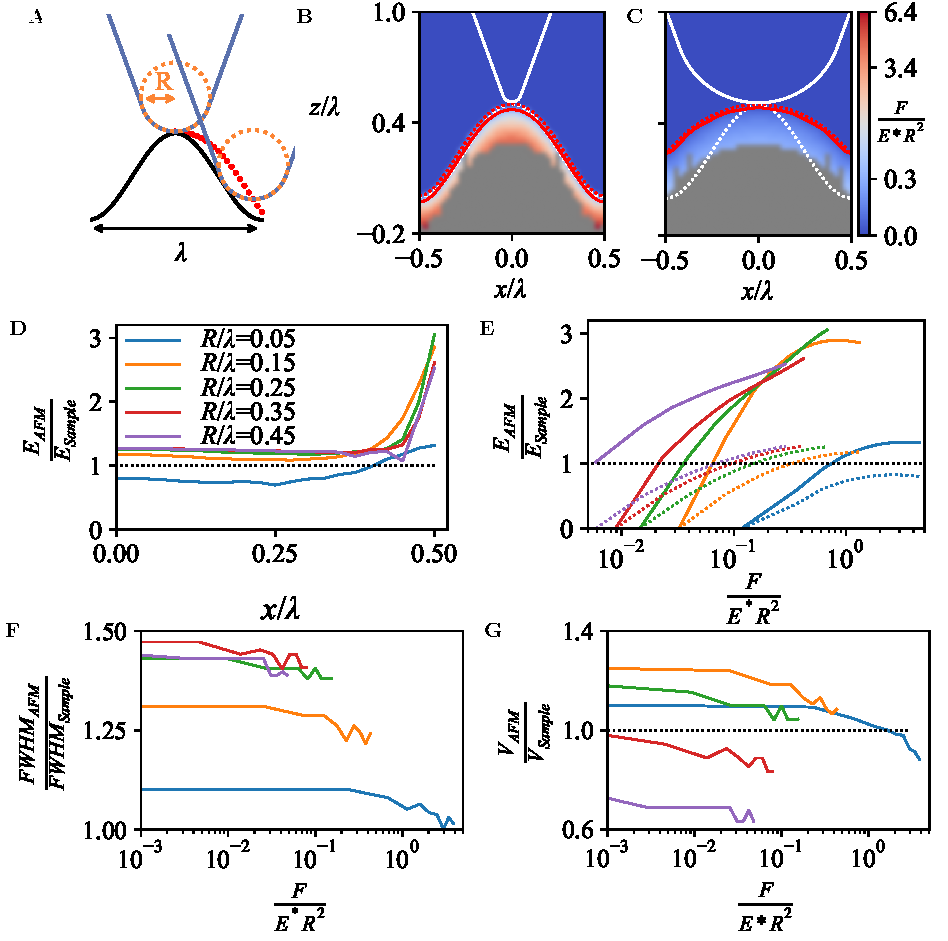
\includegraphics[width=\linewidth]{Figures/Figure4.pdf} 
    \caption{\label{fig: Wave Compression Plot}(A) Geometry of scan along the central axis of a hemisphere. Three-dimensional geometry is produced by rotating the indenter and extruding the wave. Wave is shown in black with wavelength $\lambda$. Indenter geometry is shown in blue with a circular tip of radius $R$ in orange. Red points indicate initial scan positions (Hard sphere contact points). (B) Interpolated two-dimensional heat map of indentation force over the scanning axis for periodic structure with indenter $R/\lambda=0.05$. Including overlayed contour of constant force, $\frac{F}{E^*R^2} = 0.227 $, shown in solid red. The indenter is solid white, and the surface is dotted white. Points of zero force/ hard sphere contact are shown in dotted red. (C) Interpolated two-dimensional heat map of indentation force over the scanning axis for periodic structure with indenter $R/\lambda=0.45$. Including overlayed contour of constant force, $\frac{F}{E^*R^2} = 0.227 $, shown in solid red. The indenter is solid white, and the surface is dotted white. Points of zero force/ hard sphere contact are shown in dotted red. (D) Fitted Young's modulus over scan positions for each indenter radius ($R/\lambda$). (E) Apparent Young's modulus variation over contour force for each indenter radius($R/\lambda$). Measured at trough (solid line) and at crest (dashed). (F) Relative FWHM of the contour ($FWHM^*=\frac{FWHM_{AFM}}{FWHM_{Sample}}$) variation over contour force for each indenter radius($\frac{R}{\lambda}$). (G)  Volume variation over contour force in spherical structures for each indenter radius($R/\lambda$).}
    
\end{figure}


The individual contribution highlights the deviation and behaviour of the surface when indented. Figure \ref{fig: Wave FWHM/Fourier Plot}B shows an illustrative plot of the Fourier component's amplitudes for corresponding frequencies. The zeroth component of the Fourier series represents a linear vertical offset. The increasing trend corresponds to an increased trough height for larger indenter-surface ratios. The first component corresponds to surface periodicity and is expected for the contours that match the surface's geometry ($A_k = 1$ for $k=1$ and zero for $k\neq 1$), as shown by the black bar. The decreasing amplitude of this component corresponds to an increase in surface distortion, as the amplitude is shared proportionally with higher-order terms. The second component is the significant component producing the widening wave peak, and higher-order terms refine the curvature of the contour.

Therefore, the deviation from the true surface geometry and accuracy of the imaging can be quantified by analysing the variation of the first Fourier component over a range of contour forces. Analysing the absolute A1 for each contour force, shown in \ref{fig: Wave FWHM/Fourier Plot}C, indicates how well we extract information from the surface topography. A lower indenter-surface ratio produces less apparent structure deviation as the scan/tip more closely follows the surface geometry. Moreover, A1 is generally constant over the range of contour forces. 

In contrast, the relative variation of higher order component $\sum^N_{k>1} A_k$, shown in Figure \ref{fig: Wave FWHM/Fourier Plot}D, indicates that although the relative value of the first component may be constant throughout the forces range, the percentage of anomalous higher order terms in the series does decrease. As these higher-order terms are linked to errors in contour shape, this suggests a greater percentage of the periodicity of the surface is recovered. This indicates that the apparent resolution extracted from the AFM image increases with indentation force. This could be due to the increased proportion of the indenter in contact with the surface and the elastic behaviour becoming more linear for deeper/high-force indentations. As a result, the indentations are subject to more influence from the surfaces and better resolved topological variation. 

Overall, this illustrates how strongly the measured topography and nanomechanics may depend on tip and sample geometry and the applied forces in an AFM experiment. As before, the volume highlights that the larger indenters/contact areas require larger forces to compress the sample to the same extent as smaller indenters. However, the Fourier analysis elucidates a possible novel feature, demonstrating that larger indentation forces recover more surface periodicity.

\begin{figure}[htp]
    \centering
    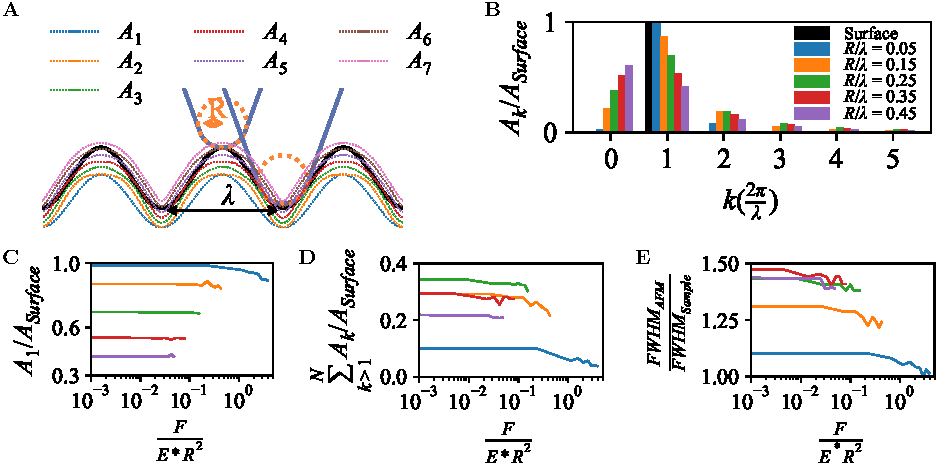
\includegraphics[width=\linewidth]{Figures/Figure5.pdf} 
    \caption{\label{fig: Wave FWHM/Fourier Plot}Analysis of force contours for a periodic structure. (A) Geometry of scan along the central axis of a hemisphere. Three-dimensional geometry is produced by rotating the indenter and extruding the wave. Wave is shown in black with wavelength $\lambda$. Indenter geometry is shown in blue with a circular tip of radius $R$ in orange. Illustration of Fourier decomposition for hard sphere contour show as dashed lines. (B) Fourier Series Component for force contours at $\frac{F}{E*R^2} = 0.227$. (C) Variation of relative component $A_1/A_{Sample}$ over contour force for a range of indenters ($\frac{R}{\lambda}$). (D) Relative variation of higher order component $\sum^N_{k>1} A_k$ over contour force for range of indenters ($\frac{R}{\lambda}$). (E) Variation of relative FWHM over contour force for each indenter radius($\frac{R}{\lambda}$).}  
\end{figure}